\documentclass[border=4pt]{standalone}
\usepackage{amsmath,amssymb,tikz}\usetikzlibrary{arrows.meta}
\definecolor{figB}{RGB}{31,90,166}\definecolor{figR}{RGB}{176,48,48}\definecolor{figG}{RGB}{46,125,50}\definecolor{figO}{RGB}{214,120,20}
\begin{document}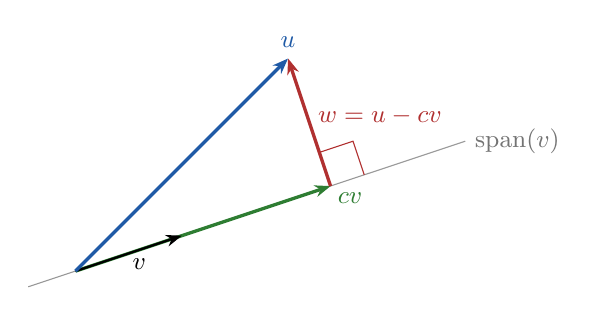
\begin{tikzpicture}[scale=1.5,>={Stealth[length=2mm]}]
\draw[black!40] (-0.4,-0.133)--(3.3,1.1) node[right,font=\small,black!55]{$\operatorname{span}(v)$};
\draw[->,very thick,figG] (0,0)--(2.16,0.72) node[below right,font=\small,inner sep=2pt]{$cv$};
\draw[->,thick] (0,0)--(0.9,0.3) node[pos=0.6,below,font=\small,inner sep=3pt]{$v$};
\draw[->,very thick,figB] (0,0)--(1.8,1.8) node[above,font=\small]{$u$};
\draw[figR] (2.16,0.72) ++(-0.0949,0.2846) -- ++(0.2846,0.0949) -- ++(0.0949,-0.2846);
\draw[->,very thick,figR] (2.16,0.72)--(1.8,1.8) node[pos=0.55,right,font=\small]{$w=u-cv$};
\end{tikzpicture}\end{document}
